% Created 2020-01-30 Thu 09:51
% Intended LaTeX compiler: pdflatex
\documentclass[presentation]{beamer}
\usepackage[utf8]{inputenc}
\usepackage[T1]{fontenc}
\usepackage{graphicx}
\usepackage{grffile}
\usepackage{longtable}
\usepackage{wrapfig}
\usepackage{rotating}
\usepackage[normalem]{ulem}
\usepackage{amsmath}
\usepackage{textcomp}
\usepackage{amssymb}
\usepackage{capt-of}
\usepackage{hyperref}
\usepackage{minted}
\usetheme{Singapore}
\author{Julius (juliuss@u.nus.edu)}
\date{\today}
\title{CS2040S Tutorial 1}
\hypersetup{
 pdfauthor={Julius (juliuss@u.nus.edu)},
 pdftitle={CS2040S Tutorial 1},
 pdfkeywords={},
 pdfsubject={},
 pdfcreator={Emacs 26.3 (Org mode 9.2.1)}, 
 pdflang={English}}
\begin{document}

\maketitle

\section{Introduction}
\label{sec:org0de242e}
\begin{frame}[<+->][label={sec:orgd454d8a}]{About me}
\begin{itemize}
\item Year 3 in CS (Interest in Distributed Systems)
\item Did CVWO for the past 2 summers
\item Uses Emacs
\end{itemize}
\end{frame}
\begin{frame}[label={sec:org0d5804a}]{Now your turn!}
\begin{itemize}
\item Name
\item Interests (Preferably not CS related)
\item What was the nicest thing you ate over CNY?
\end{itemize}
\end{frame}
\begin{frame}[<+->][label={sec:orgabbdc2e}]{What to expect}
\begin{itemize}
\item CS2040S is intense
\begin{itemize}
\item Some of the material is new to me!
\end{itemize}
\item Prepare for class
\item Contribute to class
\item I try to respond to emails in like \textasciitilde{}24 hours
\begin{itemize}
\item Or you can ping our Telegram group - others probably have the
same query!
\end{itemize}
\item I don't want to touch code!
\end{itemize}
\end{frame}

\section{Java}
\label{sec:org924694f}
\begin{frame}[label={sec:org1457884}]{Classes and Objects}
\begin{itemize}
\item What is a class?
\item What is an object?
\end{itemize}
\end{frame}
\begin{frame}[label={sec:orgdea3e97},fragile]{Classes and Objects}
 \begin{minted}[]{java}
class Student {
  private String name;

  public Student(String name) {
    this.name = name;
  }
}

Student hans = new Student("Hans");
\end{minted}
\end{frame}
\begin{frame}[label={sec:orgb47c110},fragile]{Classes and Objects}
 \begin{minted}[]{java}
class Student {
  private static String name;

  public Student(String name) {
    this.name = name;
  }
}

Student hans = new Student("Hans");
\end{minted}
\end{frame}

\begin{frame}[label={sec:org6f59d48},fragile]{Classes and Objects}
 \begin{minted}[]{java}
class Student {
  private String name;

  public Student(String name) {
    this.name = name;
  }

  private void sayName() {
    System.out.printf("Hi, my name is %s\n", this.name);
  }
}

Student hans = new Student("Hans");
hans.sayName();
\end{minted}
\end{frame}
\begin{frame}[<+->][label={sec:org04728ef}]{Java vs Source}
\begin{block}{Object-orientedness}
Everything in Java is an object (well, mostly).
\end{block}
\begin{block}{Immutability}
Because of the object-oriented nature of Java, immutability
often isn't guaranteed.
\end{block}
\begin{block}{Higher Order Functions}
It's a pain in Java (Covered in CS2030).
\end{block}
\end{frame}
\begin{frame}[label={sec:orgaac7719},fragile]{Pass by value vs pass-by-reference}
 \begin{minted}[]{java}
class X { String n = "hi"; }

void foo(X x) {
  x.n = "bye";
}

X x = new X();
foo(x);
System.out.println(x.n);
\end{minted}
\end{frame}
\begin{frame}[label={sec:org6d97732},fragile]{Pass by value vs pass-by-reference}
 \begin{minted}[]{java}
class X { String n = "hi"; }

void goo(X x) {
  x = new X();
  x.n = "bye";
}

X xx = new X();
goo(xx);
System.out.println(xx.n);
\end{minted}
\end{frame}
\begin{frame}[label={sec:org5b6c2b1},fragile]{Pass by value vs pass-by-reference}
 \begin{minted}[]{java}
void hoo(int x) {
  x += 3;
}

int n = 3;
hoo(n);
System.out.println(n);
\end{minted}
\end{frame}
\section{Complexity}
\label{sec:org7d31b4b}
\begin{frame}[<+->][label={sec:org1194392}]{Formulas}
\begin{itemize}
\item \(f_1(n) = 7.2 + 34n^3 + 3254n\)
\item \(f_2(n) = n^2\log{n} + 25n\log^2{n}\)
\item \(f_3(n) = 2^{4\log{n}} + 5n^5\)
\item \(f_4(n) = 2^{2n^2 + 4n + 7}\)
\end{itemize}
\end{frame}
\begin{frame}[<+->][label={sec:orgd88a56e}]{Formulas}
Let \(f\) and \(g\) be functions of \(n\) where \(f(n) = O(n)\) and \(g(n) =
O(\log n)\).  
\begin{itemize}
\item \(h_1(n) = f(n) + g(n)\)
\item \(h_2(n) = f(n) \times g(n)\)
\item \(h_3(n) = \max(f(n), g(n))\)
\item \(h_4(n) = f(g(n))\)
\item \(h_5(n) = f(n)^{g(n)}\)
\end{itemize}
\end{frame}
\begin{frame}[label={sec:org9376be1},fragile,shrink=30]{Example 1}
 \begin{minted}[]{java}
public static int niceFunction(int n)
{
        for (int i = 0; i < n; i++)
        {
                System.out.println("I am nice!");
        }
        return 42;
}

public static int meanFunction(int n)
{
        if(n == 0) return 0;
        return (2 * meanFunction(n/2) + niceFunction(n));
}

public static int evilFunction(int n)
{
        for(int i = 2; i < n; i *= i){
                System.out.println("To be or not to be");
        }
        return 666;
}

\end{minted}
\end{frame}
\begin{frame}[label={sec:org4c23362},fragile]{Example 2}
 \begin{minted}[]{java}
public int strangerFunction(int n) {
  for (int i = 0; i < n; i++) {
    for (int j = 0; j < i; j++) {
      System.out.println("Execute order?");
    }
  }
  return 66;
}
\end{minted}
\end{frame}
\begin{frame}[label={sec:orgee5e06e},fragile]{Example 2}
 \begin{minted}[]{java}
public int suspiciousFunction(int n) {
  if (n == 0) return 2040;

  int a = suspiciousFunction(n / 2);
  int b = suspiciousFunction(n / 2);
  return a + b + niceFunction(n);
}
\end{minted}
\end{frame}
\begin{frame}[label={sec:org1d37768}]{Example 2}
\begin{center}
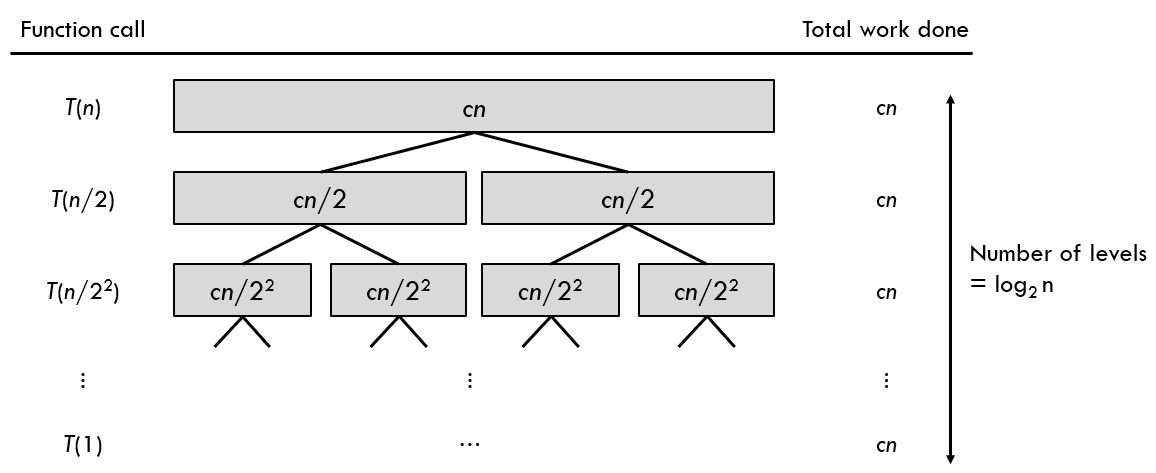
\includegraphics[width=.9\linewidth]{nlogn.png}
\end{center}
\end{frame}
\begin{frame}[label={sec:org5c4d4f7},fragile]{Example 3}
 \begin{minted}[]{java}
public int badFunction(int n) {
  if (n <= 0) return 2040;
  if (n == 1) return 2040;
  return badFunction(n - 1) + badFunction(n - 2) + 0;
}
\end{minted}
\end{frame}
\begin{frame}[label={sec:org5090b10},fragile]{Example 4}
 \begin{minted}[]{java}
public int metalGearFunction(int n) {
  for (int i = 0; i < n; i++) {
    for (int j = 1; j < i; j *= 2) {
      System.out.println("!");
    }
  }
  return 0;
}
\end{minted}
\end{frame}
\section{Binary Search}
\label{sec:org6e99100}
\begin{frame}[<+->][label={sec:org9c6066c}]{When can we use binary search?}
\begin{itemize}
\item Increasing/decreasing sequence of numbers
\item Can we think of a more general criteria?
\item Think about the peakfinding algorithm
\end{itemize}
\end{frame}
\begin{frame}[label={sec:org7f1b26b}]{A more general criteria}
\begin{itemize}
\item Given a sequence of elements \(E = [e_{1}, e_{2}, ..., e_{j}]\)
\item Want to find element \(e^{*}\) in \(E\)
\item \(\exists f\), such that \(\forall i, f(e_{i})\) can tell us:
\begin{itemize}
\item if \(e_{i}\) is \(e^{*}\), or
\item \(e^{*}\) is in \([e_{1}, e_{2}, ... e_{i - 1}]\), or
\item \(e^{*}\) is in \([e_{i+1}, e_{i+2}, ... e_{j}]\)
\end{itemize}
\end{itemize}
\end{frame}
\begin{frame}[label={sec:org89b94a4}]{Example: Normal Binary Search}
\begin{itemize}
\item Find \(5\) in [1,2,4,5,6,7]
\item \(E = [1,2,4,5,6,7]\)
\item \(f(x) =\)
\begin{itemize}
\item found if \(x = 5\),
\item search in \([1,2,...,x - 1]\) if \(x > 5\),
\item search in \([x + 1, x+2...]\) if \(x < 5\)
\end{itemize}
\end{itemize}
\end{frame}

\begin{frame}[<+->][label={sec:org8024717}]{Example: Peakfinding}
\begin{itemize}
\item Find \alert{peak} in [1,2,4,5,2,3].
\item \(f(x) = ?\)
\begin{itemize}
\item \(f(x) = \frac{d}{dx}(x)\)
\item found if \(f(x) = 0\),
\item search in \([1,2,...,x - 1]\) if \(f(x) < 0\),
\item search in \([x + 1, x+2...]\) if \(f(x) > 0\)
\end{itemize}
\item \(E = ?\)
\item \(E = [[-\infty, 1, 2], [1,2,4], [2,4,5], [4,5,2],[5,2,3],[2,3,\infty]]\)
\end{itemize}
\end{frame}
\begin{frame}[<+->][label={sec:orga3167d5}]{Peakfinding Implementation}
\begin{itemize}
\item \(\texttt{map(E)}\) takes \(O(n)\)
\item Lazy evaluation
\item \(f(x)\) is an operation where \(x\) is an index perhaps?
\end{itemize}
\end{frame}

\begin{frame}[label={sec:org9a2f652},fragile]{Binary search skeleton}
 \begin{minted}[]{python}
def binary_search(arr, f):
  mid = len(arr) / 2
  if f(mid) == FOUND:
    return mid
  elif f(mid) == LEFT:
    # don't actually do this in python
    return binary_search(arr[:mid-1], f)
  else:
    return binary_search(arr[mid+1:], f)
\end{minted}
\begin{itemize}
\item By reducing the algorithm to its simplest elements, we can ease
our implementation
\end{itemize}
\end{frame}
\begin{frame}[label={sec:org8be1cd3}]{Let's try out today's problem}
(Refer to Tutorial Sheet)
\end{frame}
\begin{frame}[label={sec:org50fbd87}]{Invariants \& Inductive properties}
\begin{block}{At \emph{any} point of the execution you're at}
\begin{itemize}
\item What can we say about our array?
\item What can we say about \alert{indices}?
\end{itemize}
\end{block}
\end{frame}
\begin{frame}[label={sec:org31f99a6}]{Summary}
\begin{block}{Java}
\begin{itemize}
\item OOP properties
\end{itemize}
\end{block}
\begin{block}{Binary search}
\begin{itemize}
\item Removing edge cases
\item Abstracting reusable elements
\end{itemize}
\end{block}
\end{frame}
\begin{frame}[<+->][label={sec:orgb88bf83},fragile]{To think about}
 \begin{itemize}
\item Your brother comes to you with a corrupted hard disk, such that any
bit until position \(x\) is safe, but not the rest.
\item The good news: you have a hard disk debugger that tells you at a
position \(p\):
\begin{itemize}
\item \texttt{TRUE} if the bit at \(p\) is safe,
\item \texttt{FALSE} if the bit at \(p\) is either corrupted or not in the hard disk.
\end{itemize}
\item The bad news: your brother forgot how big his hard disk is
\item How can we find \(x\)?
\end{itemize}
\end{frame}
\end{document}